%% This is an example first chapter.  You should put chapter/appendix that you
%% write into a separate file, and add a line \include{yourfilename} to
%% main.tex, where `yourfilename.tex' is the name of the chapter/appendix file.
%% You can process specific files by typing their names in at the 
%% \files=
%% prompt when you run the file main.tex through LaTeX.
\chapter{Conceptos preliminares}

En el diseño de software y hardware para sistemas complejos, cada vez es más el tiempo y esfuerzo dedicado a la verificación en vez de la construcción. Se buscan técnicas para reducir y facilitar el trabajo de la verificación y a la vez incrementar su cobertura. Los métodos formales ofrecen un gran potencial para obtener una integración temprana de la verificación en el proceso de diseño, para proveer técnicas de verificación mas efectivas, y para reducir el tiempo de verificación en general.\\
\\
La verificación de modelos o \emph model \emph checking es una técnica automática de verificación de propiedades sobre sistemas con una cantidad finita de estados. Es una alternativa interesante con respecto al testing o las simulaciones ya que a diferencia de estas técnicas, el model checking hace una prueba exhaustiva del sistema, es decir, analiza todas las trazas posibles de la ejecución del sistema en cuestión. Sin embargo, esto trae un problema, esto es el problema de la explosión de estados. Esto ocurre en sistemas con muchas interacciones internas, y que pueden hacer crecer exponencialmente el espacio de estados posibles del sistema, ya que la prueba es exhaustiva no se puede ignorar ningún estado posible. En los últimos años se ha logrado un gran progreso en cómo lidiar con este problema mediante formas más compactas de representar al sistema, como por ejemplo, una representación simbólica del modelo del sistema \cite{Bryant:8} \cite{Burch:4}.\\
\\
El modelo del sistema generalmente es generado automáticamente desde una descripción del modelo en un un lenguaje similar a alguno de programación como C, Java, etc. Hay que notar que la especificación de la propiedad prescribe lo que el sistema debe y no debe hacer, en cambio la descripción del modelo señala como se comporta el sistema. El verificador de modelos examina todos los estados relevantes del sistema para verificar si satisface o no la propiedad deseada. El proceso del verificación de modelos consta de varias fases diferenciables \cite{Baier:2}:\\
\\
Modelado: Hay que modelar el sistema en cuestión usando el lenguaje de descripción de modelos del verificador, y formalizar la propiedad que se desea verificar usando el lenguaje de especificación de propiedades.\\
\\
Ejecución: Ejecutar el verificador para corroborar la validez de la propiedad en el modelo del sistema.\\
\\
Análisis: Si la propiedad fue satisfecha, verificar la próxima propiedad (si la hay), si en cambio, no fue satisfecha, hay que refinar el modelo y/o la propiedad y finalmente, repetir el proceso.\\

\section{Ventajas y desventajas de la verificación de modelos}
Ventajas de la verificación de modelos \cite{Baier:2}:\\
\\
- Es un enfoque general de verificación que es aplicable a una gran variedad de areas, como sistemas embebidos, ingenieria de software, y diseño de hardware.\\
\\
- Soporta verificación parcial, por lo tanto permite enfocarse en las propiedades escenciales primero.\\
\\
- No es vulnerable a la probabilidad de que un error sea expuesto, en contraste con el testing y la simulación que son técnicas que apuntan a escenarios particulares de error.\\
\\
- Provee información en caso de que una propiedad sea inválida, lo çuál es útil para el $debugging$.\\
\\
- La utilización de un verificador necesita poca interacción con el usuario.\\
\\
- Esta creciendo en popularidad debido a su facilidad de uso.\\
\\
- Tiene una base matemática, se basa en teoria de grafos, estructuras de datos y lógica, lo cuál la hace confiable.\\
\\
Desventajas de la verificación de modelos \cite{Baier:2}:\\
\\
- Es principalmente apropiada para aplicaciones dirigidas por control y menos apropiada para aplicaciones dirigidas por datos ya que los datos suelen pertenecer a dominios infinitos.\\
\\
- Su aplicación esta sujeta a problemas de decidibilidad; para sistemas de estados infinitos, la verificación de modelos en general no es efectivamente computable.\\
\\
- Verifica un modelo del sistema, en vez del sistema real mismo, cualquier resultado obtenido es tan bueno como el modelo del sistema.\\
\\
- Solo verifica los requisitos que se hayan descripto, es decir, no hay garantia de completitud.\\
\\
- Sufre del problema de la explosión de estados, ya que la cantidad de estados necesarios para modelar el sistema puede facilmente exceder la memoria disponible de la computadora. Si bien hay formas de combatir este problema (ver capítulo 3), los modelos de sistemas reales aun asi suelen ser demasiado grandes.\\
\\
- Su utilización requiere conocimiento sobre como abstraer un sistema para obtener un modelo adecuado, ademas de conocimientos sobre la lógica utilizada para la especifición de propiedades.\\
\\
- No garantiza resultados correctos, como cualquier herramienta, el verificador puede contener errores de software.\\
\\
- En general, verificar sistemas con una cantidad arbitraria de componentes, o sistemas parametrizados, no es posible.\\
\\
\section{Modelado de sistemas}
En esta sección veremos cómo representar un modelo explícitamente mediante una estructura de Kripke, en el siguiente capítulo veremos otra forma de representación llamada simbólica que representa el modelo mediante una fórmula lógica de primer orden.\\
\\
Sea $AP$ un conjunto de proposiciones atómicas, una estructura de Kripke $M$ sobre $AP$ es una cuatro-upla $M = (S, S_{0}, R, L)$ donde \cite{Clarke:1}: \\
\\
1. $S$ es un conjunto finito de estados.\\
\\
2. $S_{0} \in S$ es el conjunto de estados iniciales.\\
\\
3. $R \in S \times S$ es una relación de transición total, es decir para cada estado $s \in S$ existe un estado $s' \in S$ tal que $R(s,s')$ vale.\\
\\
4. $L \colon S \to 2^{AP}$ es una función que etiqueta a cada estado con el conjunto de proposiciones atómicas que son verdaderas en ese estado.\\
\\
Un camino en la estructura $M$ desde un estado $s$ es una secuencia infinita de estados $p = s_{0}, s_{1}, s_{2}, s_{3}, ...$, tal que $s = s_{0}$ y $R(s_{i},s_{i+1})$ vale para todo $i>0$.\\
\\
Sea $V = {v_{1}, v_{2}, ..., v_{n}}$ el conjunto de variables del sistema y sea $D$ el dominio, llamaremos una valuación de $V$ a una función que asocia a cada variable de $V$ un valor de $D$.\\
\\
Un estado del sistema se puede representar como una valuación de las variables del sistema. Una proposición atómica de la forma $v = d$ donde $v \in V$ y $d \in D$ será verdadera en un estado $s$ si y solo si $s(v) = d$.\\
\\
Dada una valuación, podemos escribir una fórmula que sea verdadera precisamente para esa valuación, por ejemplo si tenemos $V = \{x,y,z\}$ y la valuación $(x \gets True, y \gets True, z \gets False)$ entonces derivamos la fórmula $(x \land y \land !z)$. En general, una fórmula puede ser verdadera para varias valuaciones. Si adoptamos la convención de que una fórmula representa el conjunto de todas las valuaciones que la hacen verdadera, entonces podremos describir ciertos conjuntos de estados como fórmulas de primer orden. En particular, el conjunto de los estados iniciales del sistema puede describirse como una fórmula de primer orden $S_{0}$ sobre las variables en $V$.\\
\\
Una transición del sistema se puede representar como un par ordenado de valuaciones, de forma similar podemos describir conjuntos de transiciones mediante una formula para ese par, pero para poder expresar la fórmula se necesita una copia $V'$ de $V$ para hablar de siguiente estado, en $V'$ todas las variables estan primadas. Por ejemplo si tenemos una transición $(x \gets True, y \gets True, z \gets False,(x \gets True, y \gets True, z \gets True))$, podemos derivar la fórmula $(x \land y \land !z \land x' \land y' \land z')$.\\
\\
Consideremos el siguiente ejemplo, tenemos $V = \{x,y,z\}$ y $D = \{True, False\}$, $S_{0} (x,y,z) = (x= True \land y = True \land z = False)$, y tenemos solo una transición: $z := x \land y$,consideremos False = 0 y True = 1 por una cuestión de facilidad de lectura. Definimos asi la estructura de kripke (\ref{fig:kripke1})  de la siguiente manera:

\[S = D \times D \times D\]
\[S_{0} = \{(1, 1, 0)\}\]
\[R = \{((1, 1, 0), (1, 1, 1)), ((1, 1, 1), (1, 1, 1))\}\]
\[L (1, 1, 0) = \{x = 1, y = 1, z = 0\},\]
\[L (1, 1, 1) = \{x = 1, y = 1, z = 1\}\]

El único camino posible en esta estructura partiendo del estado inicial es: (1, 1, 0), (1, 1, 1), (1, 1, 1), (1, 1, 1) …

\begin{figure}[h!]
  \centering
  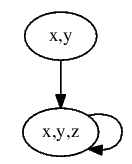
\includegraphics[width=0.2\textwidth]{Figures/kripke.png}
  \caption{Estructura de Kripke para este ejemplo.}
  \label{fig:kripke1}
\end{figure}

\section{Especificación de propiedades}

Ahora describiremos una lógica para especificar propiedades deseadas en una estructura de Kripke u otra máquina de transición de estados. La lógica utiliza proposiciones atómicas y operadores como la disyunción y la negación para construir expresiones más complicadas que describan propiedades sobre estados.
La lógica temporal es un formalismo que permite describir secuencias de transiciones entre estados en un sistema reactivo, nos interesa saber si en algún momento se llega a un estado determinado o que nunca se llegue a un deadlock. Para esto introduce nuevos operadores especiales que permiten hablar sobre tiempo. Estos operadores pueden combinarse con los operadores lógicos conocidos.
Con el propósito de familiarizarnos con las lógicas temporales, introduciremos ahora las lógicas LTL (Linear Temporal Logic), CTL (Computational Tree Logic), y CTL*. 

\subsection{CTL}

CTL tiene dos clases de fórmulas, fórmulas de estado y fórmulas de camino. Las primeras son aserciones respecto de las proposiciones atómicas en los estados y de su estructura de ramificación, mientras que las formulas de camino expresan propiedades temporales de caminos.
Las fórmulas de estado CTL sobre el conjunto AP de proposiciones atómicas, están formadas de acuerdo a la siguiente gramática\cite{Baier:2}:
\[\Phi ::= true | a | \Phi_{1} \land \Phi_{2} | \neg \Phi | \exists \varphi | \forall \varphi  \]
donde $a \in AP$ y $\varphi$ es una fórmula de camino. La sintaxis de fórmula de camino CTL esta dada por la siguiente gramática:
\[\varphi ::= \bigcirc \Phi | \Phi_{1} \cup \Phi_{2} \]
donde $\varphi$ es una fórmula de camino, y $\Phi$, $\Phi_{1}$, $\Phi_{2}$ son fórmulas de estado.

Intuitivamente $\exists f$ vale en un estado $s$, ssi a partir del mismo existe un camino donde vale f (notar que f solo puede ser una formula de estado). Naturalmente $\forall f$ significa que en todos los caminos vale f. En cuanto a $\bigcirc f$, esto vale en el camino $p$ ssi en el próximo estado (en un camino, existe un único próximo estado) vale f, y $ f\  \cup \ g$ vale en $p$ solo ssi $f$ vale siempre hasta que valga $g$. Los operadores de camino solo toman fórmulas de estado.

Los operadores booleanos $false$, $\lor$ y $\to$ se definen de la manera usual. Las modalidades temporales “eventualmente” y “siempre” pueden ser derivadas de la siguiente manera:\\
\\
eventualmente:\\
\\
$\exists \Diamond \Phi \ = \ \exists(true\ \cup \ \Phi)$\\
$\forall \Diamond \Phi \ = \ \forall(true\ \cup \ \Phi)$\\
\\
siempre:\\
\\
$\exists \Box \Phi \ = \ \neg \forall \Diamond \neg \Phi$\\
$\forall \Box \Phi \ = \ \neg \exists \Diamond \neg \Phi$\\
\\
Ejemplos de fórmulas CTL:\\
\\
$\forall \Box (\neg crit_{1} \lor \neg crit_{2})$ (exclusión mutua).\\
$\forall \Box (amarillo \lor \forall \bigcirc \neg rojo)$ (cada fase de luz roja es precedida por una fase de luz amarilla”).

\subsection{CTL*}

CTL* es una lógica que permite combinar libremente los operadores de CTL, por lo cuál CTL* incluye a CTL.
Las fórmulas de estado CTL* sobre el conjunto AP de proposiciones atómicas, están formadas de acuerdo a la siguiente gramática\cite{Baier:2}:
\[\Phi ::= true | a | \Phi_{1} \land \Phi_{2} | \neg \Phi | \exists \varphi \]
donde $a \in AP$ y $\varphi$ es una fórmula de camino. La sintaxis de fórmula de camino CTL* esta dada por la siguiente gramática:
\[\varphi ::= \Phi | \varphi_{1} \land \varphi_{2} | \neg \varphi | \bigcirc \varphi | \varphi_{1} \cup \varphi_{2} \]
donde $\Phi$ es una fórmula de estado, y $\varphi$, $\varphi_{1}$, $\varphi_{2}$ son fórmulas de camino.

Analizaremos a continuación una lógica temporal llamada cálculo-$\mu$, este puede codificar (y de hecho incluye) a CTL y CTL* \cite{Emerson:16}.

\begin{figure}[H]
  \centering
  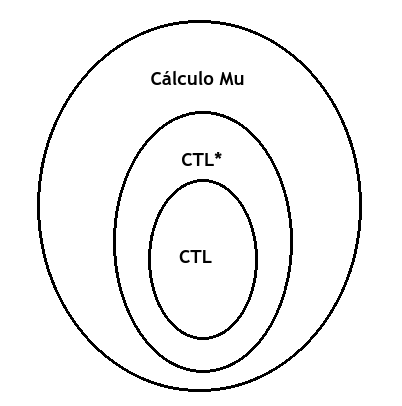
\includegraphics[width=0.6\textwidth]{Figures/inclusiontemplogic.png}
  \caption{Inclusión de lógicas temporales.} 
  \label{fig:templogics}
\end{figure}


\section{Cálculo-$\mu$}

El Cálculo-$\mu$ es un poderoso lenguaje para expresar propiedades de sistemas de transición de estados al usar operadores de punto fijo. El Cálculo-$\mu$ ha generado mucho interés entre investigadores en verificación asistida por computadoras. Este interés surge del hecho de que muchas lógicas temporales pueden ser codificadas por el Cálculo-$\mu$. Otra fuente de interés en el Cálculo-$\mu$ viene de la existencia de algoritmos eficientes de verificación de modelos para este formalismo. Como consecuencia, los procedimientos de verificación para muchas lógicas temporales y modales pueden ser descriptas al traducirse al Cálculo-$\mu$. Hay varias versiones del Cálculo-$\mu$, concretamente usaremos la versión proposicional de Kozen\cite{Kozen:3}.

\subsection{Sintaxis}

Sea $M = (S, T, L)$ una estructura de Kripke y sea $VAR = {Q, Q1, Q2, …}$ un conjunto de variables relacionales, donde a cada variable relacional se le puede asignar un subconjunto de S, construimos una $\mu$-fórmula como sigue: \\
\\
Si $p \in AP$, entonces $p$ es una fórmula. \\
\\
Si $Q \in VAR$, entonces $Q$ es una fórmula. \\
\\
Si $f$ y $g$ son fórmulas, entonces $\neg f$, $f \lor g$, y $f \land g$ son fórmulas. \\
\\
Si $f$ es una fórmula, entonces $\Box f$ y $\Diamond f$ son fórmulas. \\
\\
Si $Q \in VAR$ y $f$ es una fórmula entonces $\mu Q.f$ y $\nu Q.f$ son fórmulas. \\
\\
Las variables pueden estar libres o ligadas en una fórmula a través de un operador de punto fijo. Una fórmula cerrada es una fórmula sin variables libres.

\subsection{Semántica}

El significado intuitivo de $\Diamond f$ es “Es posible realizar una transición a un estado donde f vale“, similarmente $\Box f$ significa “f vale en todos los estados alcanzables por medio de una transición“.
Los operadores $\mu$ y $\nu$ expresan puntos fijos menores y mayores respectivamente. El conjunto vacío de estados se denota con $False$ y el conjunto de todos los estados $S$ se denota con $True$.\\
\\
Ejemplos: \\
\\
$\nu Z \cdot f \land \Box Z$ se interpreta como “f es verdadera siempre en todo camino”.\\
\\
$\mu Z \cdot f \lor \Diamond Z$ se interpreta como “existe un camino hacia un estado donde f vale”.\\
\\
$\nu Z \cdot \Diamond True \land \Box Z$ se interpreta como “no hay estados que no tengan transiciones hacia otros estados”.\\
\\
Formalmente, una fórmula $f$ se interpreta como un conjunto de estados donde $f$ es verdadera, escribimos este conjunto como $[[f]]$ sobre un sistema de transición de estados $M$ y un ambiente $e: VAR \to 2^{S}$, denotaremos $e[Q \gets W]$ como un ambiente que es igual a $e$ solo que $Q$ ahora tiene el valor $W$. el conjunto $[[f]]$ sobre $M$ y $e$ se define recursivamente de la siguiente manera:

\begin{align*}
 [[p]]\ M\ e &= \{s \mid p \in L(s)\}  \\
 [[Q]]\ M\ e &= e(Q) \\
 [[\neg f]]\ M\ e &= S \setminus [[f]]\ M\ e \\
 [[f \land g]]\ M\ e &= [[f]]\ M\ e \cap [[g]]\ M\ e \\
 [[f \lor g]]\ M\ e &= [[f]]\ M\ e \cup [[g]]\ M\ e \\
 [[\Diamond f]]\ M\ e &= \{s \mid \exists t : s \to t \land t \in [[f]]\ M\ e\} \\
 [[\Box f]]\ M\ e &= \{s \mid \forall t : s \to t  \rightarrow t \in [[f]]\ M\ e\} \\
\end{align*}
$[[\mu Q. f]] \ M\ e\ $ es el menor punto fijo del predicado transformador $t:2^{S} \to 2^{S}$ definido como $t(W) = [[f]]\ M\ e[Q \gets W] $ \\
$[[\nu Q. f]] \ M\ e\ $ es el mayor punto fijo del predicado transformador $t:2^{S} \to 2^{S}$ definido como $t(W) = [[f]]\ M\ e[Q \gets W] $ \\
\\
Observemos algunos ejemplos, supongamos que tenemos una estructura de Kripke $M = (S,T,L)$ como la de la figura \ref{fig:kripke3}, donde $L(s_{0}) = \{p,q,r\}$, $L(s_{1}) = \{p,q\}$, $L(s_{2}) = \{q,r\}$ y $L(s_{3}) = \{r\}$. Algunos ejemplos de propiedades que uno podria querer verificar son $q \land r$, $\Diamond q$, $\Box r$, $\mu Q. (r \land \neg p \lor \Diamond Q)$, $\nu Q. (p \land \Box Q)$. $q \land r$ se cumple en $\{s_{2}\}$, $\Diamond q$ se cumple en $\{s_{0},s_{1},s_{3}\}$, $\Box r$ se cumple en $\{s_{1},s_{2},s_{3}\}$, $\mu Q. (r \land \neg p \lor \Diamond Q)$ se cumple en $S$, y $\nu Q. (p \land \Box Q)$ se cumple en $\oslash$. Para entender cómo funcionan los operadores de punto fijo consideremos la fórmula $\nu Q. (p \land \Box Q)$, es decir, queremos saber que estados cumplen con la propiedad de que p vale siempre en todo camino. Cada iteración del operador esta ilustrada en la figura \ref{fig:kripke3-gfp1}. Q se inicializa en True, luego en cada iteración se hace una aproximación al resultado verdadero, los resultados de cada iteración en este caso son, en orden, $S$, $\{s_{0},s_{1}\}$, $\{s_{0}\}$, $\oslash$. Como se puede apreciar en el resultado, no hay estado donde valga esta propiedad. Si, en vez de usar el mayor punto fijo usaramos el menor, el procedimiento es análogo, solo que la variable se inicializaria en False, aunque no es dificil darse cuenta que no tiene mucho sentido verificar $\mu Q.(p \land \Box Q)$.

\begin{figure}[h!]
  \centering
  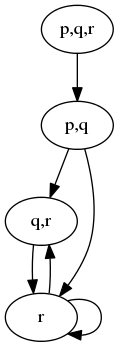
\includegraphics[width=0.2\textwidth]{Figures/kripke3.png}
  \caption{Ejemplo de Estructura de Kripke.} 
  \label{fig:kripke3}
\end{figure}
\begin{figure}[H]
  \centering
  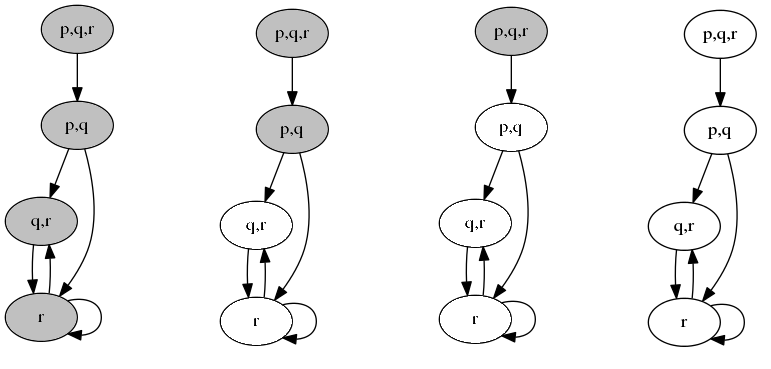
\includegraphics[width=1\textwidth]{Figures/kripke3-gfp1.png}
  \caption{Ejecución de operador de punto fijo mayor.} 
  \label{fig:kripke3-gfp1}
\end{figure}

\subsection{Algoritmo de verificación de modelos explícitos}

El algoritmo de verificación de modelos explícitos para Cálculo-$\mu$ que analizaremos es el más intuitivo (hay algoritmos mas eficientes), se basa en la semántica anterior, y calcula el subconjunto de estados de un modelo $M$ que cumplen con una formula $f$. El algoritmo trabaja en forma bottom-up a través de la fórmula, evaluandola a partir de los valores de sus subfórmulas. Este algoritmo requiere tiempo $O(n^{k})$, donde $n$ es la cantidad de estados del sistema y $k$ es el número de operadores de punto fijo anidados en la fórmula. Esto se debe a que cada operador de punto fijo hace $n+1$ iteraciones cómo máximo, ya que en cada iteración se hace una aproximación del resultado ya sea agregando o quitando al menos un estado(menor y mayor punto fijo respectivamente). En la figura \ref{fig:eval1} se puede ver el algoritmo \cite{Clarke:1}, donde $f$ es la fórmula y $e$ es el ambiente de variables relacionales.

\begin{figure}[h!]
  \centering
  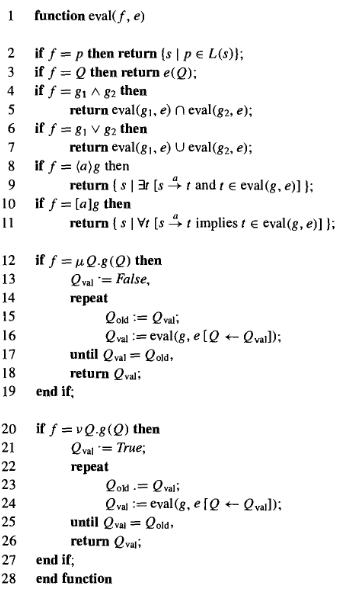
\includegraphics[width=0.7\textwidth]{Figures/eval.png}
  \caption{Algoritmo de verificación de modelos explícitos para Cálculo-$\mu$.} 
  \label{fig:eval1}
\end{figure}
